\documentclass[UKenglish]{article}  %% ... or USenglish or norsk or nynorsk
\usepackage[latin1]{inputenc}         %% ... or utf8 or applemac
\usepackage[T1]{fontenc,url}
\usepackage{mathtools}
\usepackage{listings}
\lstset{
language=JAVA,
basicstyle=\small\sffamily,
numbers=left,
numberstyle=\tiny,
frame=tb,
columns=fullflexible,
showstringspaces=false
}
\usepackage{caption}
\usepackage{graphicx}
\urlstyle{sf}
\usepackage{babel,textcomp,csquotes,varioref,graphicx}
\usepackage{amsthm}

%\usepackage[backend=biber,style=numeric-comp]{biblatex}

\title{INF5040 Assignment 3}        %% ... or whatever

%\subtitle{Increasing QoE with SDN and NFV}         %% ... if any
\author{Ida Marie Froseth}                      %% ... or whoever

%\bibliography{mybib}                  %% ... or whatever

\begin{document}
%\ififorside{}
%\cleardoublepage{}
\maketitle{}
\cleardoublepage{}
\tableofcontents{}
\cleardoublepage{}
%\listoffigures{}
%\listoftables{}

\section{Introduction}


\subsection{Average path length}
The average path length is a metric of the number of hops to reach nodes from a given sources. Hence a small average path length is preferred. As figure \ref{fig:starPL} and \ref{fig:ringPL} shows, has the star topology defenitly the best average path length. This is reasonable because a perfect star would have maximum two hops for each node. While a ring topology will have a larger average path length. When there is more and more nodes added as neighbors the path length will decrease. 
\begin{figure}
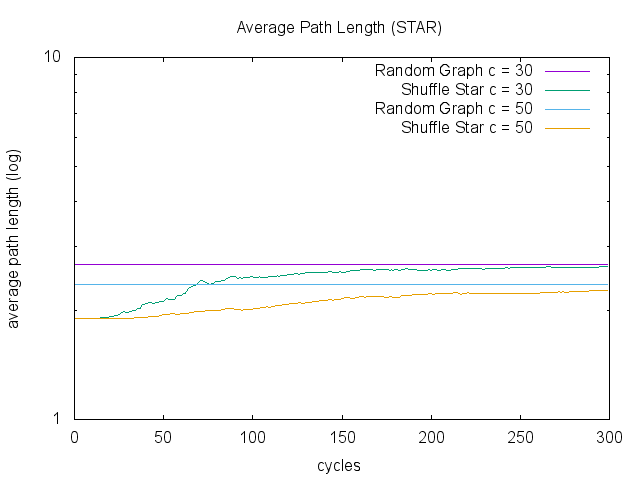
\includegraphics[scale=0.6]{plot/starPL.png}
	\caption{Star PL}
	\label{fig:starPL}
\end{figure}

\begin{figure}
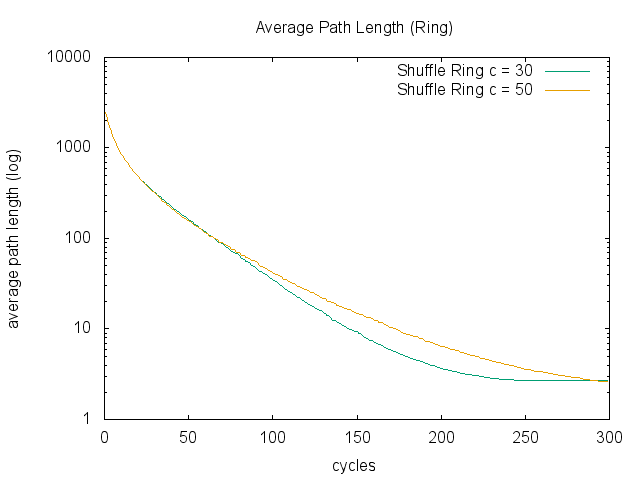
\includegraphics[scale=0.6]{plot/ringPL.png}
	\caption{Ring PL}
	\label{fig:ringPL}
\end{figure}


\subsection{Average clustering coefficient}
The clusering coefficient shows to what precentage the neighbors of a node are also neighbors among themselves. A high average clutstering indicates higher chances of network partitioning and high number of redundant message deliveries. As figure \ref{fig:ringCC} and \ref{fig:starCC} shows will both topology have a high clustering coefficient in the beginning of the shuffel exchange, while the more cycles it runs, the better. It also shows that having a larger cache actually is worse then having small cache. Comparing the the two topologies shows that also for the clustering coefficient is the star topology better to bootstrap. 
\begin{figure}
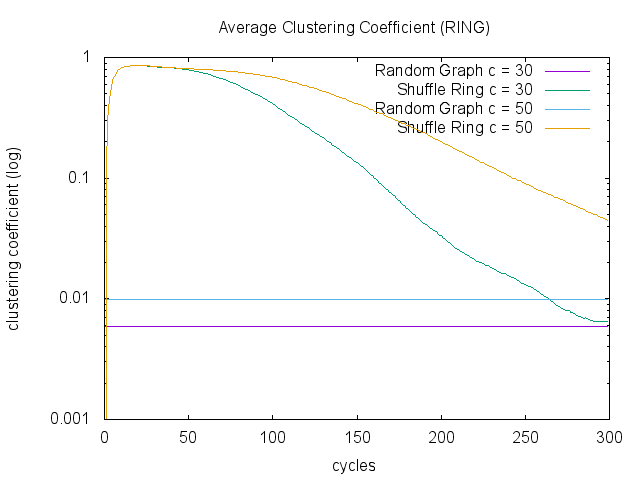
\includegraphics[scale=0.6]{plot/ringCC.png}
	\caption{Ring CC}
	\label{fig:ringCC}
\end{figure}

\begin{figure}
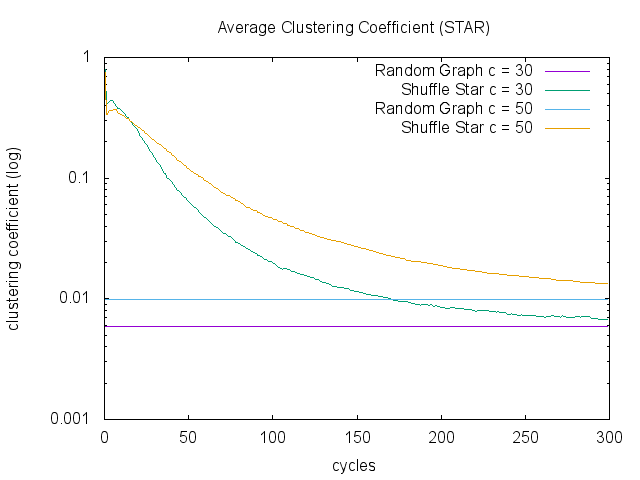
\includegraphics[scale=0.6]{plot/starCC.png}
	\caption{Star CC}
	\label{fig:starCC}
\end{figure}


\subsection{In-degree distribution}
The in-degree of a node is number of linkes it has to other nodes. High in-degree will indicate a robust network. Figure \ref{fig:ringDD} and \ref{fig:starDD} show the in-degree distribution of a ring and a star topology. As they show would for some nodes in the star topology have a very high indegree for a few nodes, typically nodes located in the center of the network. While the ring network has a gaussian distribution with the mean around the cache size, which indicates a larger cache is better. 
\begin{figure}
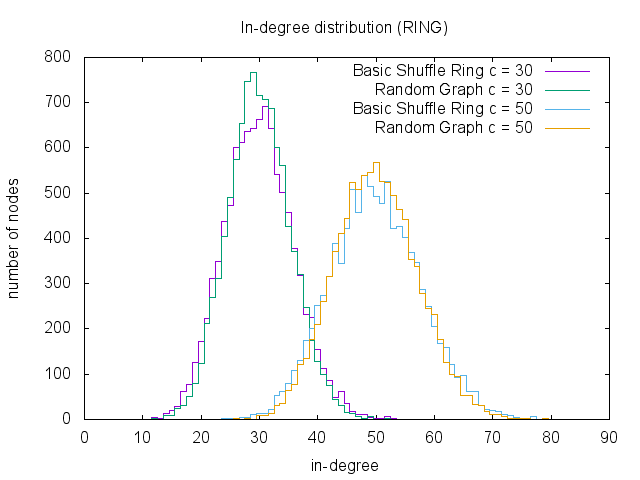
\includegraphics[scale=0.6]{plot/ringDD.png}
	\caption{Ring DD}
	\label{fig:ringDD}
\end{figure}

\begin{figure}
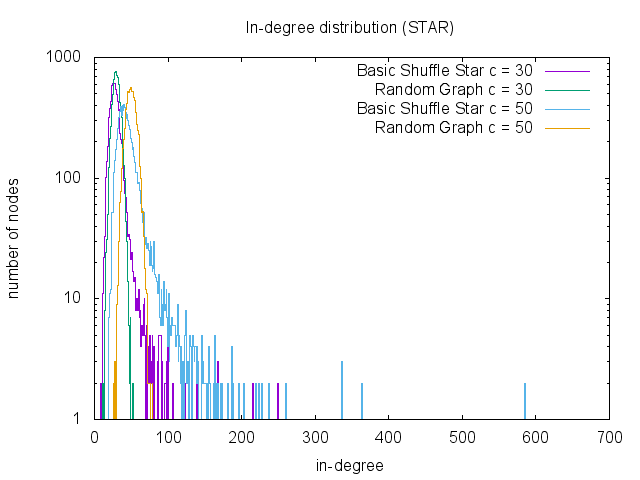
\includegraphics[scale=0.6]{plot/starDD.png}
	\caption{Star DD}
	\label{fig:starDD}
\end{figure}

\subsection{Conclusion}
From the discussed results it seems like the star topology is the best to bootstrap in such p2p system. The cache size is a trade-off, a large cache gives a high in-degree but also a slower change in the average path length and the clustering coefficient. 
\end{document}

